\documentclass[11pt]{article}
\usepackage[utf8]{inputenc}	% Para caracteres en español
\usepackage{amsmath,amsthm,amsfonts,amssymb,amscd}
\usepackage{multirow,booktabs}
\usepackage[table]{xcolor}
\usepackage{fullpage}
\usepackage{lastpage}
\usepackage{enumitem}
\usepackage{graphicx}
\usepackage{fancyhdr}
\usepackage{mathrsfs}
\usepackage{wrapfig}
\usepackage{setspace}
\usepackage{calc}
\usepackage{multicol}
\usepackage{cancel}
\usepackage[retainorgcmds]{IEEEtrantools}
\usepackage[margin=3cm]{geometry}
\usepackage{amsmath}
\newlength{\tabcont}
\setlength{\parindent}{0.0in}
\setlength{\parskip}{0.05in}
\usepackage{empheq}
\usepackage{framed}
\newcommand{\Lagr}{\mathcal{L}}
\usepackage[most]{tcolorbox}
\usepackage{xcolor}
\usepackage{pgfplots}
\pgfplotsset{compat = newest}
\usetikzlibrary{positioning, arrows.meta}
\usepgfplotslibrary{fillbetween}
\usepackage{amsmath}
\colorlet{shadecolor}{orange!15}
\parindent 0in
\parskip 12pt
\geometry{margin=1in, headsep=0.25in}
\theoremstyle{definition}
\newtheorem{defn}{Definition}
\newtheorem{reg}{Rule}
\newtheorem{exer}{Exercise}
\newtheorem{note}{Note}
\begin{document}
	\setcounter{section}{0}
	\title{Elasticity}
	\graphicspath{ {./images/} } 
	\thispagestyle{empty}
	
	\begin{center}
		{\LARGE \bf Labor Supply}\\
		{\large Economics 100A}\\
		Winter 2021
	\end{center}
	\section{Overview}
	So far, we have considered economic agents as consumers -- consumers who demand certain goods. But, are consumers also suppliers? Is it the case that consumers both supply and demand? We will set up a very interesting problem which asks this question: the Labor-Leisure problem. 
	
	Consider the following: you have some consumer who demands two goods: leisure and some composite good $x$. Let $x$ just be some representative good that the consumer demands. For this model, we want to know how some consumer chooses between supplying their labor and consuming leisure. For simplicity, let's say that time is spent either working (represented in hours by $L$) or not working (represented in hours by $Le$). In a 24-hour window, then, we can claim that $24 = L + Le$. For the general case, let $H$ denote the total time endowment in the model. We then can write more generally:
	\[T = Le + L\]
	
	Now that we have this in mind, let's proceed to our standard optimization analysis. Like in all optimization problems, we have some sort of objective function we are trying to maximize. Let's think about what choice variables we want to represent in a utility function. Does we, as consumers, consume labor?  No, not really. This would imply that you purchase labor. Instead, we can think of "consuming" leisure. Okay, so now that we have our two goods to consumer, leisure and composite good $x$, we know that our utility function will look like:
	\[u(Le, x)\]
	
	Finally, let's think about the hardest part of this problem: the constraint. What are we constraining our objective function to? Let's set up the left-hand side first. What are we consuming here? We are consuming some composite good $x$ and leisure. But what are the prices of these goods? At least for $x$, things are a bit simpler: the cost of good $x$ will just be $p_x$. The cost of leisure is a tad more complicated! Think of the price of leisure as your forgone wages. We say that if you choose to not work for an hour, this essentially costs you one hour of wages due to opportunity cost. So, the price is just wage, $w$. 
	
	Let's also look at one's income. We can say that their max income is $w$ $\times$ $H$. This is their max income if they work every single hour. We also can say that they have non-labor income (think of an allowance or a trust fund). With this being said, let's set up the budget constraint:
	\[p_x x + wLe = I_0 + wH\]
		
	Let's just set things straight now that we have everything. We recall that for consumer optimization problems, we set up the following questions:
	
	\begin{enumerate}
		\item \textbf{Objective Function}: What are we maximizing/minimizing?
		\item \textbf{Constraint}: What do we constrain our objective function to? 
		\item \textbf{Choice variables}: What variables do we choose to achieve maximization/minimization? 
		\item \textbf{Exogenous variables}: What variables affect the situation but are taken as given? 
	\end{enumerate}
	
	By now you should be able to answer all of these questions. But I will do it just in case you had trouble following the notes.  
	
	\begin{enumerate}
		\item \textbf{Objective Function}: We maximize consumer utility
		\item \textbf{Constraint}: We constrain utility to our new budget constraint relating income to leisure.
		\item \textbf{Choice variables}: We maximize utility via consuming $x$ and $Le$, so we maximize the quantity of each good. 
		\item \textbf{Exogenous variables}: We take prices, wage, and  non-labor income as given. 
	\end{enumerate}
	
	Let's write the problem as follows:
	\[max \hspace{.2cm} u(Le, x) \]
	\[ \textnormal{s.t.}  p_x x + wLe = I_0 + wH \]
	
\section{Graphical Solution} 

%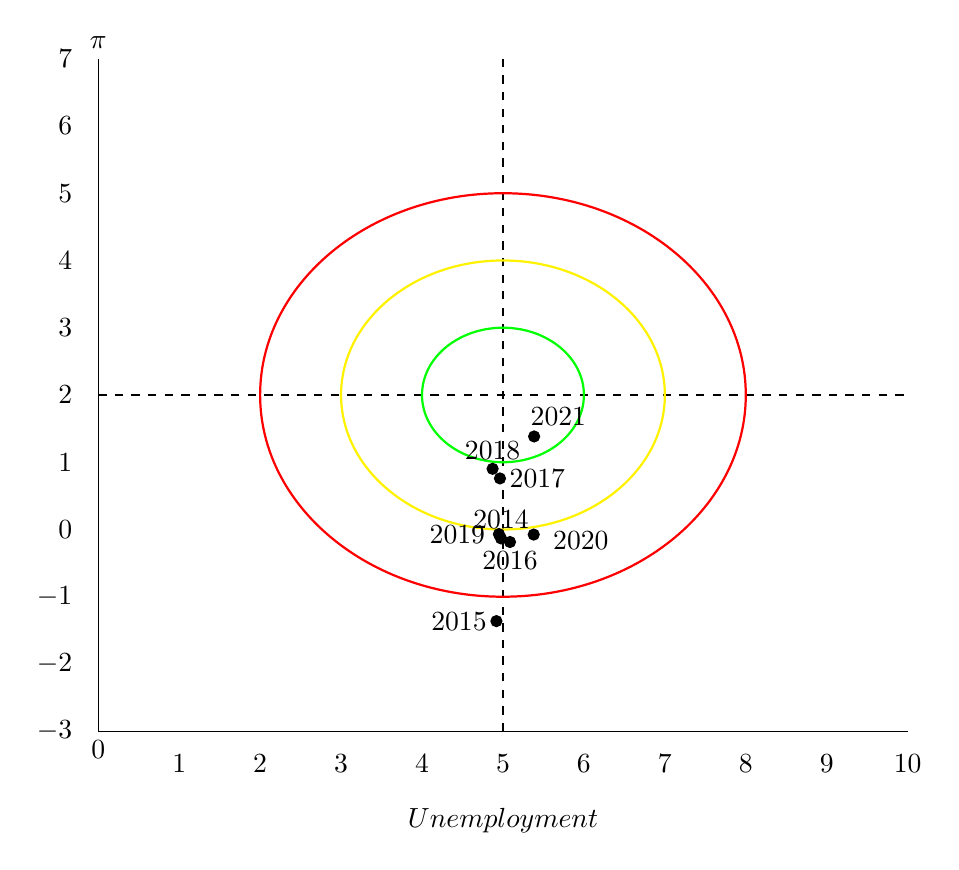
\begin{tikzpicture}
\begin{axis}[
scale = 1.5,
xmin = 0, xmax = 10,
ymin = -3, ymax = 7,
axis lines* = left,
xtick = {0}, ytick = \empty,
clip = false,
% every axis plot/.append style={ultra thick}
]
% Indifference curve
% \addplot[line width=2pt, domain = 0:20, restrict y to domain = 0:70, samples = 400, color = blue]{4-.4*x};
%\addplot[line width=1pt, domain = 0:10, restrict y to domain = 0:10, samples = 400, color = black]{(940.607/((x^3)^.5))};
%\addplot[line width=1pt, domain = 0:10, restrict y to domain = 0:10, samples = 400, color = black]{(940.607/((x^3)^.5))};


\addplot[color = black, dashed, thin] coordinates {(0, 2) (10, 2)};
\addplot[color = black, dashed, thin] coordinates {(5, -3) (5, 7)};

\draw[color=green, thick, ->] (5, 2) circle (1);
\draw[color=yellow, thick, ->] (5, 2) circle (2);
\draw[color=red, thick, ->] (5, 2) circle (3);


% \addplot[domain = 1:10, restrict y to domain = 0:10, samples = 400, color = blue]{10/(x-(.01)^2)+1};
\addplot[color = black, mark = *, only marks, mark size = 2pt] coordinates {(4.976, -.133) (4.919, -1.363) (5.087, -.1863) (4.963, .759) (4.872, .902)  (5.38, -.076) (4.95, -.069) (5.385, 1.383)  };


% Labels
\node [below] at (5, -4) {$Unemployment$};
\node [above] at (current axis.above origin) {$\pi$};
%\node [right] at (25, 9.5) {$(24, 8)$};
\node [below] at (5, -3.2) {$5$};
\node [below] at (6, -3.2) {$6$};
\node [below] at (7, -3.2) {$7$};
\node [below] at (8, -3.2) {$8$};
\node [below] at (9, -3.2) {$9$};
\node [below] at (10, -3.2) {$10$};
\node [below] at (4, -3.2) {$4$};
\node [below] at (3, -3.2) {$3$};
\node [below] at (2, -3.2) {$2$};
\node [below] at (1, -3.2) {$1$};


\node [left] at (-.2, -3) {$-3$};
\node [left] at (-.2, -2) {$-2$};
\node [left] at (-.2, -1) {$-1$};
\node [left] at (-.2, 0) {$0$};
\node [left] at (-.2, 1) {$1$};
\node [left] at (-.2, 2) {$2$};
\node [left] at (-.2, 3) {$3$};
\node [left] at (-.2, 4) {$4$};
\node [left] at (-.2, 5) {$5$};
\node [left] at (-.2, 6) {$6$};
\node [left] at (-.2, 7) {$7$};


\node [above] at (5.685, 1.4) {$2021$};
\node [left] at (4.9, -.076) {$2019$};
\node [right] at (5.5, -.169) {$2020$};

\node [above] at (4.976, -.133) {$2014$};
\node [left] at (4.919, -1.363) {$2015$};

\node [below] at (5.087, -.1863) {$2016$};
\node [right] at (4.963, .759) {$2017$};
\node [above] at (4.872, .902) {$2018$};


%\node [left] at (-1, 8) {$8$};
%\node [left] at (20, -1) {$A$};
%\node [below] at (-1, 40) {$C$};



% \node [below] at (-.75, 2) {$\frac{I}{p_2'} = 2$};
% \node [right] at (2.47 ,4) {$C$};
% \fill[orange, opacity = 0.1] (10, 1.1) -- (10, 2) -- (1, 11) -- (1, 11);
\end{axis}
\end{tikzpicture}


%Kids, turn away. We are getting graphic. 
	
\end{document}